% vim:ts=4:sw=4:expandtab
% © 2012 Michael Stapelberg
%
% use xelatex %<
%
\documentclass[xetex,serif,compress]{beamer}
\usepackage{fontspec}
\usepackage{xunicode} % Unicode extras!
\usepackage{xltxtra}  % Fixes
\usepackage{listings}
\setmainfont{Trebuchet MS}
\setmonofont{Inconsolata}
\usetheme{default}

\setbeamertemplate{frametitle}{
    \color{black}
    \vspace*{0.5cm}
    \hspace*{0.25cm}
    \textbf{\insertframetitle}
    \par
}

% Hide the navigation icons at the bottom of the page
\setbeamertemplate{navigation symbols}{}

% No margins on any side
\setbeamersize{text margin left=0cm,text margin right=0cm}


\begin{document}

% slide with bullet points
\newcommand{\mslide}[2]{
    \begin{frame}{#1}
        \begin{center}
        \begin{list}{$\bullet$}{\itemsep=1em}
            #2
        \end{list}
        \end{center}
    \end{frame}
}

\frame{
\begin{center}
\vspace{1.5cm}
{\huge i3}\\
{\large improved tiling window manager}\\
\vspace{3cm}
Michael Stapelberg\\
\vspace{0.5cm}
2012-01-25\\
\end{center}
}

\begin{frame}{}
\begin{center}
\huge
"Interesting, what is this?"

\vspace*{1cm}

vs.

\vspace*{1cm}

"What?! \textbf{Another} window manager?"
\end{center}
\end{frame}


\begin{frame}{}
    % talk about the difference between a desktop environment and a window manager:
    % a desktop environment (like GNOME, KDE, Xfce) is a collection of
    % programs, libraries (including a graphical toolkit) and configuration.
    % it usually aims for a coherent look and feel and comes with a number of
    % tools (g*, like gedit, geeqie, …)
    % One of the programs of a DE is a window manager.
    \begin{figure}
    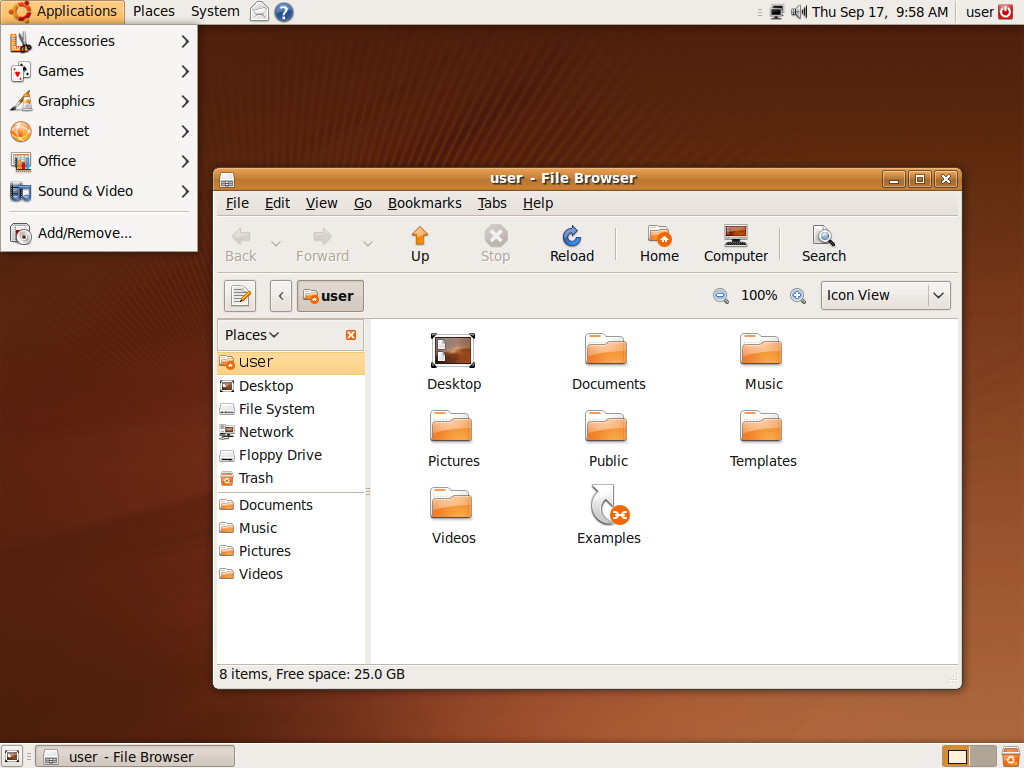
\includegraphics[width=0.97\textwidth]{Ubuntu_Linux_Jaunty_screenshot.png}
    % source: http://en.wikipedia.org/wiki/File:Ubuntu_Linux_Jaunty_screenshot.png
    \end{figure}
\end{frame}


\begin{frame}{}
\begin{center}
% compare this to a screenshot of i3:
% notice the little amount of toolbars.
% notice the lack of fancy window decorations
% notice the absence of a desktop.
% instead, you get to use the full screen.
    \begin{figure}
    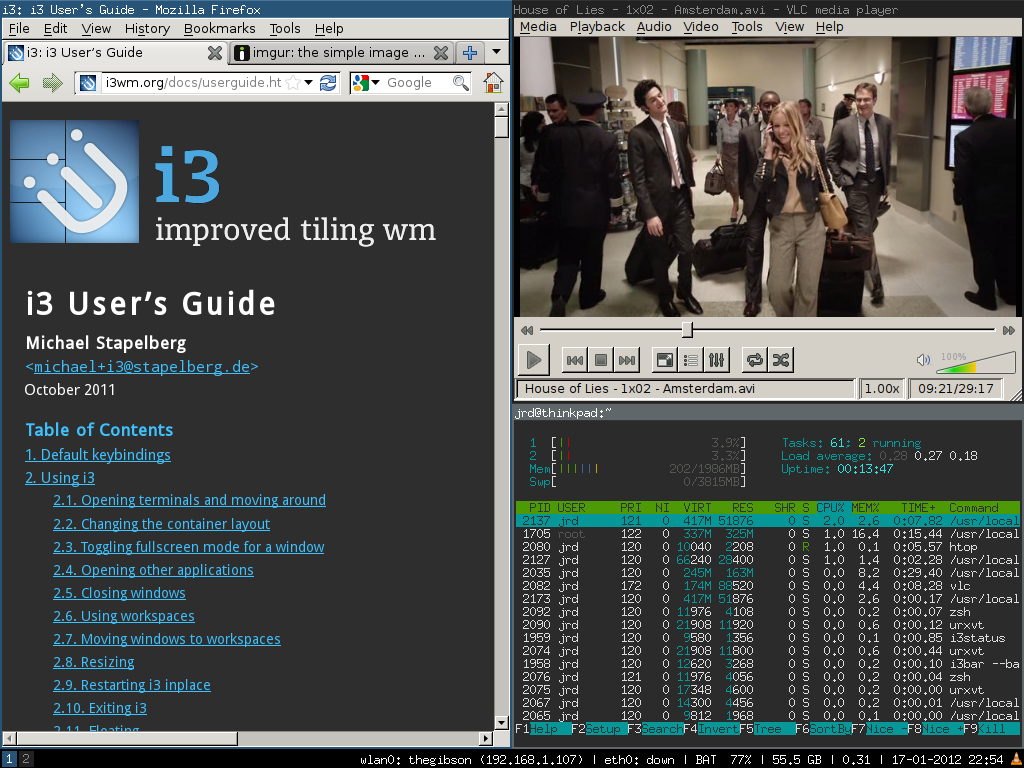
\includegraphics[width=0.97\textwidth]{TdilE.jpg}
    % source: jrd in #i3
    \end{figure}
\end{center}
\end{frame}


\mslide{i3: history and features}{
    \item started from scratch in february 2009
    \item successor* to wmii, which we couldn’t hack
    \item clean, readable, documented code. and documentation
    \item proper multi-monitor support, utf-8 clean
    \item fast and lightweight, aimed at power users
}

% live demo here, just like at FrOSCon
% include: the docs, with the keyboard layout
% include: the configuration file

\mslide{Inter-process communication}{
    \item UNIX socket, JSON for serialization
    \item i3-msg (C), AnyEvent::I3 (Perl), i3-ipc (Ruby), i3ipc (Python)
    \item send any command, like \texttt{floating enable}
    \item receive events (like focus change)
    \item access the layout tree (!)
}

% demo: change a workspace
% demo: testsuite

\mslide{Example workflows}{
    \item Urgency hint
    \item Scratchpad
    \item Web development (browser, editor, syslog)
    \item Coding (C): two editors (code, test), quickly opening docs
}

\mslide{i3 in numbers}{
    \item 3149 commits by 39 different people
    \item > 600 tickets (about 60 open)
    \item about 10.000 SLOC (mostly C, a bit of Perl)
    \item testsuite: > 1000 test instructions in 96 files
    \item conservative guess of > 1000 users
}

\mslide{Thanks for your attention}{
    \item See \url{http://www.i3wm.org/} for everything
    \item Ubuntu: upgrade to our repository: \url{http://i3wm.org/docs/repositories.html}
    \item Debian: upgrade to the version in Debian testing
    \item Any questions?
    \item (pictures Creative Commons Attribution-Share Alike 3.0 Unported)
}

\end{document}
